\documentclass[11pt,a4paper]{article}
\usepackage[top=3cm, bottom=2cm, left=2cm, right=2cm]{geometry}
\usepackage[utf8]{inputenc}
\usepackage{amsmath, amsfonts, amssymb}
\usepackage{siunitx}
\usepackage[brazil]{babel}
\usepackage{graphicx}
\usepackage[margin=10pt,font={small, it},labelfont=bf, textfont=it]{caption}
\usepackage[dvipsnames, svgnames]{xcolor}
\DeclareCaptionFont{MediumOrchid}{\color[svgnames]{MediumOrchid}}
\usepackage[pdftex]{hyperref}
\usepackage{natbib}
\bibliographystyle{plainnat}
\bibpunct{\textcolor{MediumOrchid}{\textbf{[}}}{\textcolor{MediumOrchid}{\textbf{]}}}{,}{s}{}{}
\usepackage{color}
\usepackage{footnote}
\usepackage{setspace}
\usepackage{booktabs}
\usepackage{multirow}
\usepackage{subfigure}
\usepackage{fancyhdr}
\usepackage{leading}
\usepackage{indentfirst}
\usepackage{wrapfig}
\usepackage{mdframed}
\usepackage{etoolbox}
\usepackage[version=4]{mhchem}
\usepackage{enumitem}
\usepackage{caption}
\usepackage{titlesec}
\usepackage{tcolorbox}
\usepackage{tikz}
\usepackage{LobsterTwo}
\usepackage[T1]{fontenc}
\usepackage{fontspec}
\usepackage{txfonts}
\usepackage[bottom]{footmisc}
\tcbuselibrary{skins,breakable}
\sisetup{output-decimal-marker={.}}

\makeatletter
\def\footnoterule{\kern-3pt\color{MediumOrchid}\hrule\@width0.6\textwidth height 0.8pt\kern2.6pt}
\makeatother

\renewcommand{\footnotelayout}{\itshape\color{MediumOrchid}}

\AtBeginEnvironment{equation}{\fontsize{13}{16}\selectfont}


\titleformat{\section}{\LobsterTwo\huge\color{CarnationPink}}{\thesection.}{1em}{}
\titleformat{\subsection}{\LobsterTwo\huge\color{CarnationPink}}{\thesubsection}{1em}{}
\titleformat{\subsubsection}{\bf\LobsterTwo\Large\color{MediumOrchid}}{\thesubsubsection}{1em}{}


\DeclareCaptionLabelFormat{figuras}{\textcolor{DarkTurquoise}{Figura \arabic{figure}}}
\captionsetup[figure]{labelformat=figuras}

\makeatletter
\renewcommand\tagform@[1]{\maketag@@@{\color{CarnationPink}(#1)}}
\makeatother

\renewcommand{\theequation}{Eq. \arabic{equation}}
\renewcommand{\thefigure}{Fig. \arabic{figure}}
\renewcommand{\thesection}{\textcolor{CarnationPink}{\arabic{section}}}

\setlist[itemize]{label=\textcolor{CarnationPink}{$\blacksquare$}}

\setlist[enumerate]{label=\textcolor{CarnationPink}{\arabic*.}, align=left, leftmargin=1.5cm}


\newcounter{exemplo}

\NewDocumentEnvironment{exemplo}{ O{} }{%
\allowbreak
\setlength{\parindent}{0pt}
  \begin{mdframed}[
  leftline=true,
  topline=false,
  rightline=false,
  bottomline=false,
  linewidth=2pt,
  linecolor=CarnationPink,
  frametitlerule=false,
  frametitlefont=\LobsterTwo\large\color{CarnationPink},
  frametitle={\color{CarnationPink}\LobsterTwo\large #1},
  ]
}{%
  \end{mdframed}
}

\setlength{\fboxsep}{5pt}
\setlength{\fboxrule}{1.5pt}
\usepackage{float}
\renewcommand{\thefootnote}{\alph{footnote}}
\usepackage{url}
\hypersetup{
	colorlinks=true,
	linkcolor=DarkTurquoise,
	filecolor=DarkTurquoise,      
	urlcolor=DarkTurquoise,
	citecolor=DarkTurquoise,
	pdftitle={Especialista em Física da Radioterapia}
}
\pagestyle{fancy}
\fancyhf{}
\renewcommand{\headrulewidth}{0pt}
\rfoot{\color{DarkTurquoise}\thepage \\ \LobsterTwo{\small\textcolor{CarnationPink}{@defDalila}}}
\title{\LobsterTwo\Huge{Garantia Da Qualidade}}
\author{\LobsterTwo\Large{QA em Cálculos de Dose}\nocite{*}}
\date{\LobsterTwo\textit{Dalila Mendonça}}
\begin{document}
	\maketitle

\section{Introdução}

	Na radioterapia moderna, a grande maioria dos cálculos de dose é realizada por sistemas computadorizados. Pode haver exceções menores, como radiofármacos usados em medicina nuclear. O sistema pode calcular todos ou alguns dos seguintes: \textcolor{MediumOrchid}{\textbf{\textit{doses pontuais, isodoses 2D, isodoses 3D e doses para volumes}}}. Além disso, toda uma série de informações não dosimétricas podem ser utilizadas para informar os médicos quanto à qualidade do plano de tratamento. Isso inclui informações de imagem (tomografia computadorizada (TC), ressonância magnética (RM), tomografia por emissão de pósitrons (PET), ultrassom (US) etc.), informações de imagem derivadas (visão de feixe (BEV), radiografias reconstruídas digitalmente (DRRs) ) e aberturas de feixe (estáticas e dinâmicas). A fonte de radiação pode ser produzida eletricamente (linac, ortovoltagem, ciclotron, etc.) ou de um material radioativo (\ce{^{60}Co}, \ce{^{137}Cs}, \ce{^{192}Ir}, \ce{^{125}I}, \ce{^{103}Pd}, \ce{^{223}Ra}, etc.). O termo geral para esses tipos de sistemas é sistema de planejamento de tratamento (TPS).

	Existem recomendações para QA do TPS  de várias instituições, bem como muitas fontes de dados de referência. Uma referência padrão é o TG-53 \textit{``QA for Clinical Radiotherapy Treatment Planning''}, que discute muitos dos problemas observados aqui em um nível geral.

\section{Comissionamento do TPS}

\subsection*{Testes Dosimétricos}

	Os dados dosimétricos podem estar na forma de \textcolor{MediumOrchid}{\textbf{\textit{doses pontuais, isodoses 2D, isodoses 3D, informações de dose/volume ou atividade}}}. Para testar a precisão dos cálculos de um sistema, três estratégias podem ser empregadas:

	\begin{enumerate}
		\item Comparação entre as doses calculadas e as doses medidas;
		\item Comparação entre as doses calculadas com os dados de referência;
		\item Comparação entre as doses calculadas em um sistema com as doses calculadas em outro sistema já validado.
	\end{enumerate}

	Um comissionamento completo de um sistema geralmente envolve o uso de pelo menos duas dessas estratégias.

	Outro fator que deve ser avaliado é a \textcolor{MediumOrchid}{\textbf{\textit{resolução da grade de cálculo de dose}}}. Um sistema pode fornecer resultados clinicamente diferentes para um espaçamento de grade de 4 mm em comparação com uma grade de 2 mm. É muito importante reconhecer quando usar grades menores ou maiores. Por exemplo, alguns estudos recomendam grades de 2.5 mm ou menores para cálculos de radioterapia de intensidade modulada (IMRT), e o espaçamento da grade deve ser proporcional à largura da lâmina do colimador (MLC), o que significa que um micro-MLC precisará de um espaçamento de 2 mm ou menor. Outras considerações especiais incluem o uso do \textcolor{MediumOrchid}{\textbf{\textit{planejamento de tratamento baseado em Monte Carlo}}} para contabilizar as heterogeneidades do tecido, os efeitos da dose devido aos tampos das mesas e modelos biológicos.

	O usuário deve estar ciente de como o TPS reporta a dose com respeito a heterogeneidades. O sistema pode calcular a dose para o meio ou converter a dose para a água usando razões poderes de freamento. Esses dois métodos levarão a resultados diferentes. 

	Os cálculos de Monte Carlo têm sido usados há muito tempo para calcular doses com precisão, particularmente em \textcolor{MediumOrchid}{\textbf{\textit{tecidos heterogêneos}}}, onde os \textcolor{MediumOrchid}{\textbf{\textit{problemas de transporte de elétrons não são tratados adequadamente por cálculos baseados em modelos}}}. Os longos tempos de cálculo dos algoritmos de Monte Carlo impediram seu uso generalizado na clínica. Com o advento de hardware de computação mais rápidos e códigos otimizados, eles entraram no mainstream. As questões de incerteza estatística, a capacidade de contabilizar a geometria exata do cabeçote do acelerador e outros recursos são exclusivos dos algoritmos de Monte Carlo e devem ser bem compreendidos para uma implementação precisa. Por exemplo, devido à incerteza estatística da dose para qualquer voxel, a normalização para doses pontuais pode levar a resultados inesperados. Isso é especialmente relevante para o elétron Monte Carlo, onde a dose de tratamento é frequentemente prescrita para $d_{max}$. Para prescrições de dose para uma determinada linha de isodose, uma incerteza de cálculo de Monte Carlo de 2\% na isodose de prescrição evoluiu como um padrão clínico. Deve-se notar, porém, que \textcolor{MediumOrchid}{\textbf{\textit{as incertezas do cálculo da dose são maiores para órgãos de risco (OARs) recebendo doses menores do que a dose prescrita}}}. Um sistema de planejamento de tratamento Monte Carlo deve ser capaz de exibir a incerteza do cálculo da dose no planejamento de tratamento para permitir que os médicos avaliem completamente a distribuição da dose.

	o TG-176,\textit{``Dosimetric Effects Caused by Couch Tops and Immobilization Devices''}, discute como a \textcolor{MediumOrchid}{\textbf{\textit{mesa de tratamento}}} e os \textcolor{MediumOrchid}{\textbf{\textit{acessórios de imobilização}}} podem causar \textcolor{MediumOrchid}{\textbf{\textit{aumento da dose na pele}}}, \textcolor{MediumOrchid}{\textbf{\textit{redução da dose do tumor}}} e uma \textcolor{MediumOrchid}{\textbf{\textit{alteração na distribuição da dose}}} se não forem tratados adequadamente. Em particular, \textcolor{MediumOrchid}{\textbf{\textit{a entrada do feixe através de componentes de alta densidade deve ser evitada}}}. A \textcolor{MediumOrchid}{\textbf{\textit{atenuação através das mesas de fibra de carbono}}} pode variar de 2\% para feixes com incidência normal até 6\% para feixes altamente oblíquos em baixas energias. Além disso, regiões mais densas podem causar até 17\% de atenuação. \textcolor{MediumOrchid}{\textbf{\textit{A atenuação aumentará se o tampo da mesa for emparelhado com outros dispositivos de imobilização}}}. Há casos em que a dose na pele pode atingir 100\% da dose máxima. Correções simples de atenuação podem levar a cálculos de dose imprecisos, e a \textcolor{MediumOrchid}{\textbf{\textit{inclusão explícita dos dispositivos de imobilização e da mesa no TPS é recomendada}}}.

	AAPM TG-166, \textit{``The Use and QA of Biologically Related Models for Treatment Planning''}, discute quatro questões com modelos biológicos:

	\begin{enumerate}
		\item Estratégias, limitações, condições e cuidados ao utilizar modelos biológicos;
		\item O uso prático dos modelos biológicos mais comumente usados: dose uniforme equivalente (EUD), probabilidade de complicação de tecido normal (NTCP), probabilidade de controle de tumor (TCP) e probabilidade de controle de tumor livre de complicação ($P_+$);
		\item Características desejáveis e direções futuras de modelos biológicos;
		\item Diretrizes gerais e metodologia para testes de aceite, comissionamento e controle de qualidade contínuo de modelos biológicos.
	\end{enumerate}

	Como o uso de modelos biológicos representa uma mudança de paradigma, eles devem ser implementados com cuidado para evitar uma perigosa aplicação incorreta dos modelos. \textcolor{MediumOrchid}{\textbf{\textit{O uso de modelos biológicos pode trazer vantagens tanto na otimização quanto na avaliação do plano}}}. Isso ocorre porque, se o modelo for preciso, os resultados estarão diretamente correlacionados com os desfechos do tratamento e poderão classificar os planos de forma mais confiável para um determinado paciente.

\subsection*{Comparação das Doses Calculadas Com as Doses Medidas}

	O Medical Physics Practice Guideline (MPPG) 5 da AAPM sobre Comissionamento e QA de TPS em terapia com feixe externo, tem um resumo dos requisitos mínimos para testes dosimétricos (AAPM TG-244). O teste não dosimétrico não faz parte do escopo do documento planejado.

	Ao comissionar um TPS, existem dois tipos de medidas realizadas:

	\begin{enumerate}[label=\textcolor{CarnationPink}{\roman*.}]
		\item Dados do feixe necessários para caracterizar o modelo de feixe; e
		\item Dados necessários para validar o modelo;
	\end{enumerate}

	Para aceleradores lineares, este é o assunto abordado no TG-106 \textit{``Accelerator Beam Data Commissioning Equipment and Procedure''}. O conjunto de caracterização varia de acordo com o fornecedor, mas inclui itens como fatores de output, fatores de transmissão dos filtros em cunha, curvas de dose na profundidade e de perfis. Estes são normalmente medidos em um phantom de água. O usuário deve ter o cuidado de realizar as medidas nas condições descritas pelo fornecedor. Uma atenção especial deve ser dada à \textcolor{MediumOrchid}{\textbf{\textit{definição da condição de normalização}}} e à \textcolor{MediumOrchid}{\textbf{\textit{definição da transmissão dos filtros em cunha}}}. Por exemplo, alguns sistemas normalizam para a SSD de 90 cm e 10 cm de profundidade, enquanto outros requerem uma SSD de 100 cm. Além disso, alguns sistemas requerem transmissão do filtro em cunha em relação a um campo de 10 cm x 10 cm, enquanto outros requerem uma relação do filtro em cunha com respeito a um aberto para cada tamanho de campo que for medido.

	A medida da \textcolor{MediumOrchid}{\textbf{\textit{dose na superfície}}} deve ser feita usando o detector apropriado (uma câmara de extrapolação ou câmara de placas paralelas). Esta é tipicamente uma região de fraqueza para muitos algoritmos de cálculo de dose e deve ser avaliada com cuidado. \textcolor{MediumOrchid}{\textbf{\textit{Se o sistema não puder calcular com precisão a dose na superfície, podem ser necessárias medidas mais frequentes paciente-específico para confirmar a dose na pele}}}.

	As \textcolor{MediumOrchid}{\textbf{\textit{doses fora de campo}}} são importantes para caracterizar o risco de situações como \textcolor{MediumOrchid}{\textbf{\textit{gestantes}}} e pacientes com \textcolor{MediumOrchid}{\textbf{\textit{dispositivos eletrônicos implantados}}}. TG-158, \textit{``Measurements and Calculations of Doses Outside the Treatment Volume from External Beam Radiation Therapy''}, aborda recomendações nesta área. A precisão das medidas de dose fora de campo deve ser verificada usando um phantom antropomórfico. Nos últimos anos, alguns estudos clínicos surgiram enfatizando a importância de avaliar a dose integral e a dose em órgãos distantes para evitar cânceres secundários tardios. Estudos demonstraram que alguns sistemas podem ter dificuldade em calcular essas doses com precisão. \textcolor{MediumOrchid}{\textbf{\textit{Em distâncias próximas ao volume irradiado, o espalhamento interno é o maior componente da dose, enquanto em distâncias maiores o espalhamento da máquina e a fuga predominam}}}. Para sistemas \textcolor{MediumOrchid}{\textbf{\textit{conformacionais 3D}}}, o \textcolor{MediumOrchid}{\textbf{\textit{espalhamento interno}}} contribui com até 70\% da dose e é a \textcolor{MediumOrchid}{\textbf{\textit{componente dominante  até 25 cm do volume irradiado}}}. Para \textcolor{MediumOrchid}{\textbf{\textit{IMRT,}}} o \textcolor{MediumOrchid}{\textbf{\textit{espalhamento interno é dominante apenas até 10 cm do volume irradiado}}}, com o espalhamento do colimador dominando os próximos 10 cm e a fuga do cabeçote além de 20 cm.

	O conjunto de validação é um conjunto mais extenso de medidas que abrange a gama de situações clínicas que se espera ser utilizadas naquela unidade. Isso incluirá \textcolor{MediumOrchid}{\textbf{\textit{dados de dose na profundidade e dados de perfil para várias SSDs, dados de ângulo oblíquo, efeito de não homogeneidade e modelagem de campos complexos}}}. 

	Ao realizar essas medidas, muitos métodos podem ser usados. O mais básico é o uso dos detectores apropriados em um phantom de água. \textcolor{MediumOrchid}{\textbf{\textit{O phantom de água pode adquirir dados 1D e dados de dose pontual}}}. Da mesma forma, phantom sólidos podem ser usados em combinação com dosímetros pontuais. O dosímetro pontual é, na verdade, um dosímetro de volume (muito pequeno), portanto, o usuário deve garantir que o dosímetro seja apropriado para os gradientes e tamanhos de campo usados.

	Usando uma \textcolor{MediumOrchid}{\textbf{\textit{combinação de placas de materiais água-equivalentes e não equivalentes, os efeitos de heterogeneidades podem ser analisados}}}. Devido às alterações no espectro do feixe e nas propriedades de espalhamento dentro ou perto de materiais não aquosos, pode ser necessário fazer \textcolor{MediumOrchid}{\textbf{\textit{correções nas leituras do dosímetro}}}. Para \textcolor{MediumOrchid}{\textbf{\textit{filme}}} embutido em material não aquoso, \textcolor{MediumOrchid}{\textbf{\textit{a dose medida é a dose para o filme}}}, não a dose para a falta de homogeneidade. A comparação pode ser feita usando a dose em água para o cálculo ou aplicando a correção apropriada à medição usando relações de poder de freamento. As medidas da câmara de ionização precisarão de correções semelhantes.

	\textcolor{MediumOrchid}{\textbf{\textit{Filmes e  matriz de detectores}}} podem ser utilizados para \textcolor{MediumOrchid}{\textbf{\textit{medir dados 2D}}}. O filme tem a vantagem de uma \textcolor{MediumOrchid}{\textbf{\textit{resolução espacial muito maior}}}, mas pode ser problemático ao tentar medir campos maiores. A maioria dos departamentos de radioterapia não possui mais processadores de filme, então o filme radiocrômico é utilizado ao invés de filmes radiográficos. \textcolor{MediumOrchid}{\textbf{\textit{Os scanners usados para analisar filmes radiocrômicos sofrem de falta de uniformidade na resposta em áreas maiores}}}, o que limita a precisão dos resultados. As \textcolor{MediumOrchid}{\textbf{\textit{matrizes de detectores}}} têm uma \textcolor{MediumOrchid}{\textbf{\textit{boa uniformidade na resposta em áreas maiores}}}, mas sofrem de \textcolor{MediumOrchid}{\textbf{\textit{baixa resolução espacial}}}. Os detectores estão situados na matriz a uma distância de 5 a 10 mm, dependendo do modelo exato utilizado. Também pode haver diferenças de resposta direcional. Esses detectores podem ser usados para avaliar efeitos de heterogeneidade, mas são limitados a \textcolor{MediumOrchid}{\textbf{\textit{dados de transmissão}}}, pois seu design não permite que eles meçam dentro ou próximo a uma falta de homogeneidade.

\subsection*{Heterogeneidade do Tecido no Cálculo de Dose no TPS}

	Alguns sistemas usarão um \textcolor{MediumOrchid}{\textbf{\textit{número CT (HU)}}} para curva de correção de densidade criada usando a densidade física, enquanto outros usam \textcolor{MediumOrchid}{\textbf{\textit{densidade eletrônica}}}. Nem todos os algoritmos de cálculo de dose funcionam igualmente dentro e ao redor das heterogeneidades do tecido, e o usuário deve estar ciente das incertezas e limitações do algoritmo. O TG-65, \textit{``Tissue Inhomogeneity Corrections for Megavoltage Photon Beams''}, apresenta uma avaliação detalhada das correções de heterogeneidades. Ele descreve o desempenho de diferentes algoritmos em várias condições e apresenta recomendações. Um resumo das recomendações são:

	\begin{enumerate}[label=\textcolor{CarnationPink}{\roman*.}]
		\item \textcolor{DarkTurquoise}{\textbf{\textit{As correções de heterogeneidade devem ser aplicadas aos cálculos de dose e prescrições}}}. Mesmo que haja imprecisões no algoritmo, ele estará mais próximo da realidade do que se nenhuma correção for aplicada.
		
		\item Para \textcolor{DarkTurquoise}{\textbf{\textit{tratamentos de cabeça e pescoço, laringe e pulmão}}}, até mesmo algoritmos simples calcularão adequadamente em áreas distantes das interfaces óssea e aérea. Perto dessas interfaces, os algoritmos de Convolução e de Monte Carlo terão um desempenho melhor. Para materiais de alta densidade eletrônica, o AAPM TG-63, \textit{`` Dosimetric Considerations for Patients with Hip Prostheses Undergoing Pelvic Irradiation''}, fornece detalhes.
		
		\item Para \textcolor{DarkTurquoise}{\textbf{\textit{tratamentos pulmonares}}}, energias de 12 MV ou menores são recomendadas.
		
		\item Para \textcolor{DarkTurquoise}{\textbf{\textit{tratamentos de mama}}}, as doses perto da interface parede torácica/pulmão são calculadas com mais precisão com algoritmos de Convolução e de Monte Carlo.
		
		\item Para \textcolor{DarkTurquoise}{\textbf{\textit{tratamentos gastrointestinais}}}, as áreas de contraste de bário devem ser contornadas e a densidade deve ser substituída.
		
		\item Para \textcolor{DarkTurquoise}{\textbf{\textit{tratamentos de próstata e pelve}}}, a principal preocupação é com próteses de quadril com alta densidade eletrônica. (TG-63)
	\end{enumerate}

	O cálculo da dose para estruturas diferentes de água é realizado usando os números de HU da TC de planejamento para levar em conta as diferenças de densidade. Normalmente, um \textcolor{MediumOrchid}{\textbf{\textit{TPS usará uma tabela armazenada para converter o número de HU em densidade}}}. Esta tabela é estabelecida pela varredura de phantoms com materiais de densidade conhecida e correlacionada com os números de HU medidos. Essa relação entre densidade e número de HU depende do \textcolor{MediumOrchid}{\textbf{\textit{kVp utilizado na aquisição das imagens de referência}}} e pode ser \textcolor{MediumOrchid}{\textbf{\textit{diferente de scanner para scanner}}}, mesmo utilizando o mesmo kVp. \textcolor{MediumOrchid}{\textbf{\textit{A estabilidade dessa relação deve ser verificada ao longo do tempo e quando o tubo de TC for substituído}}}.

	Uma maneira de estabelecer os \textcolor{MediumOrchid}{\textbf{\textit{níveis de tolerância}}} para esta medida de QA é observando as aplicações clínicas típicas. A maioria dos tecidos é quase equivalente à água, portanto, para estabelecer uma faixa clinicamente relevante, você pode \textcolor{MediumOrchid}{\textbf{\textit{alterar a densidade de um phantom de água e observar quando a dose calculada a 20 cm de profundidade muda em mais de 1\%}}}. Para \textcolor{MediumOrchid}{\textbf{\textit{densidades mais baixas}}}, como pulmão, uma espessura típica é de cerca de \textcolor{MediumOrchid}{\textbf{\textit{15 cm}}}. Os níveis de tolerância podem ser calculados colocando um ponto de cálculo distal ao volume pulmonar e alterando novamente a densidade até que a dose mude em 1\%. \textcolor{MediumOrchid}{\textbf{\textit{Não se espera que as regiões de alta densidade excedam 4 cm de espessura}}}, podendo ser essa a espessura utilizada para estabelecer os níveis de tolerância para essas estruturas. O uso dessa metodologia produz intervalos de $\pm$20 HU para valores de baixa densidade e $\pm$ 100 para valores de alta densidade. Em comparação, o AAPM TG-66, \textit{``Quality Assurance for Computed-Tomography Simulators and the Computed-Tomography Simulation Process''}, \textcolor{MediumOrchid}{\textbf{\textit{recomenda um valor genérico de $\pm$5 em toda a faixa de números de HU}}}.

	Outro problema com as conversões de número de HU para densidade é o \textcolor{MediumOrchid}{\textbf{\textit{número de bits usados para armazenar os dados de TC}}}, ou seja, valores de tons de cinza. O uso de um\textcolor{MediumOrchid}{\textbf{\textit{armazenamento tradicional de 12 bits truncará os dados em um número HU de aproximadamente 3.000 (parecendo que saturou na região)}}}, enquanto o armazenamento de 16 bits permitirá valores muito mais altos ($\sim 32000$). Isso fornecerá uma dosimetria mais precisa e uma melhor visualização.

\subsection*{Comparação das Doses Calculadas com os Valores de Referência}

	Existem muitas fontes de dados de referência que detalham um parâmetro específico para comparação como \textcolor{MediumOrchid}{\textbf{\textit{fatores de output, uma compilação de dados ou planos de teste}}}. A \ref{fig:benchmarkdata} resume parte da literatura. O \textit{Imaging and Radiation Oncology Core em Houston (IROC-H)}, anteriormente conhecido como Radiological Physics Center (RPC), possui documentação sobre dados padrão para vários modelos de aceleradores lineares para feixes de fótons e elétrons. O AAPM TG-67, \textit{``Benchmark Datasets for Photon Beams''}, produziu um relatório descrevendo o conteúdo de um conjunto de dados de referência de feixe de fótons. Com base neste relatório, foi concedido um subsídio para Small Business Innovation Research (SBIR) para medir os conjuntos de dados. A Sun Nuclear Corporation recebeu esta concessão e mantém os dados. O fornecedor também pode fornecer dados de referência. Isso deve ser usado apenas para comparação e não substitui as medidas locais. \textcolor{MediumOrchid}{\textbf{\textit{O uso de dados do fornecedor como dados clínicos só deve ser feito após a validação da precisão de 1\% a 2\%}}}.

	\begin{figure}[h]
		\centering
		\subfigure{
			\fcolorbox{DarkTurquoise}{white}{%
				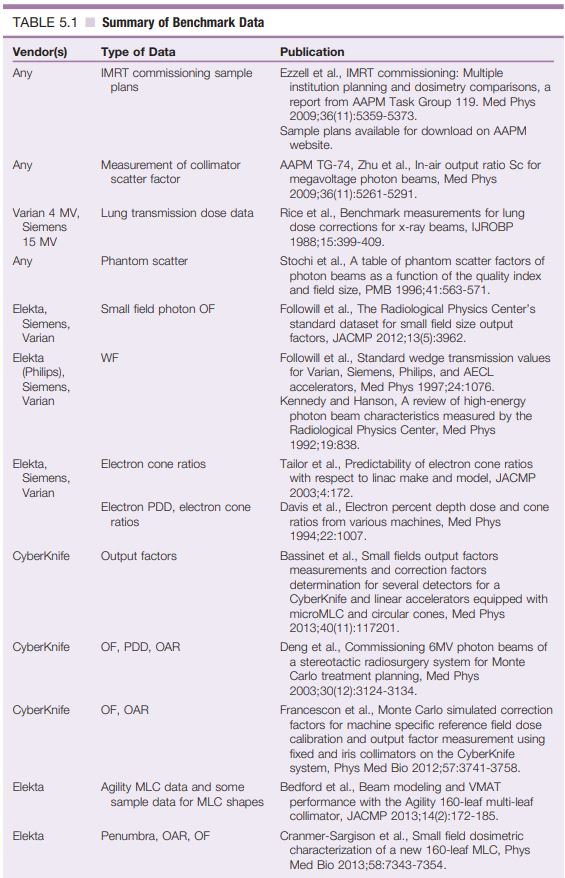
\includegraphics[width=0.4\textwidth]{Imagens/benchmarkdata1.JPG}
			}}
		\subfigure{
			\fcolorbox{DarkTurquoise}{white}{%
				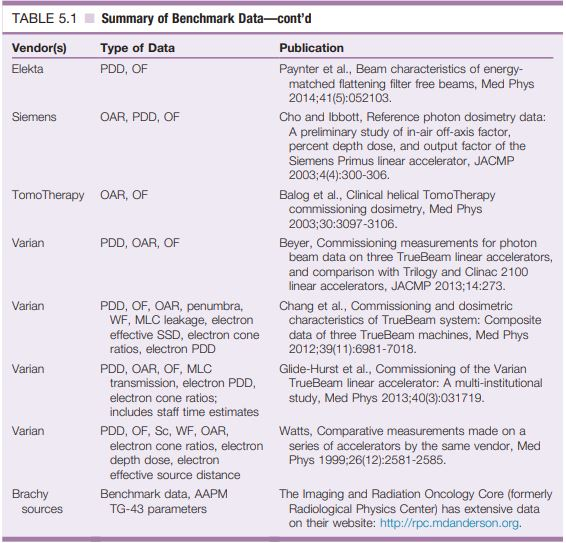
\includegraphics[width=0.4\textwidth]{Imagens/benchmarkdata2.JPG}
			}} \\ %
		\caption{Dados de Referência}
		\label{fig:benchmarkdata}
	\end{figure}

	Os dados de referência de fontes de braquiterapia estão disponíveis para fontes específicas dos fornecedores. A metodologia geral de cálculo é descrita no AAMP TG-43, \textit{``Dosimetry of Interstitial Brachytherapy Sources''} e seus suplementos.

\subsection*{Comparação das Doses Calculadas em um Sitema com as Doses Calculadas por Outro Sistema Validado}

	Este é um processo relativamente simples com várias ressalvas:
	
	\begin{enumerate}[label=\textcolor{CarnationPink}{\arabic*${}^\circ $}]
		\item \textcolor{DarkTurquoise}{\textbf{\textit{As limitações do sistema validado devem ser conhecidas}}}. Por exemplo, seriam esperadas diferenças ao comparar um modelo de convolução com um modelo de feixe tipo lápis, e a comparação não seria válida para cálculos de heterogeneidades. Nesse caso, uma comparação poderia ser feita para cálculos simples em água, mas as medidas teriam que ser feitas para situações mais complexas.
		\item \textcolor{DarkTurquoise}{\textbf{\textit{As capacidades dos dois sistemas podem não ser correspondentes entre si}}}. Por exemplo, o sistema mais novo pode ter terapia de arco volumétrico (VMAT), enquanto o mais antigo não.
		\item \textcolor{DarkTurquoise}{\textbf{\textit{Este tipo de comparação é de uso limitado para o comissionamento dosimétrico}}}. No entanto, é um processo valioso revisar com a equipe clínica quaisquer diferenças entre os sistemas para que os resultados possam ser correlacionados com a experiência anterior. 
	\end{enumerate}
	
	Como mencionado anteriormente, \textcolor{MediumOrchid}{\textbf{\textit{as diferenças nos cálculos de heterogeneidades devem ser entendidas, bem como as diferenças de penumbra podem afetar a seleção do tamanho do campo}}}. Um dos exemplos mais comuns disso é a verificação do cálculo da MU do TPS.  O TG-114, \textit{``Verification of Monitor Unit Calculations for Non-IMRT Clinical Radiotherapy''}, descreve como realizar esta verificação em detalhes. Normalmente, \textcolor{MediumOrchid}{\textbf{\textit{os dados do plano de tratamento são transferidos para um sistema independente}}} usando o protocolo DICOM (Digital Imaging and Communications in Medicine). Dependendo do sistema, o arquivo de plano, arquivos de imagem e conjuntos de estrutura podem ser transferidos. Alguns sistemas calculam o MU apenas com base na \textcolor{MediumOrchid}{\textbf{\textit{profundidade efetiva do ponto de referência e o padrão de fluência do campo de tratamento}}}. Outros sistemas realizarão \textcolor{MediumOrchid}{\textbf{\textit{um re-cálculo completo, incluindo histogramas dose-volume (DVHs)}}} para comparação. É típico que os \textcolor{MediumOrchid}{\textbf{\textit{sistemas de segunda verificação usem os mesmos dados de input}}} do feixe que o TPS comissionado. Isso irá acelerar o processo de implementação; no entanto, um controle de qualidade rigoroso do segundo sistema de verificação ainda precisa ser executado.

\subsection*{Testes End-To-End}

	Os testes End-To-End (E2E ``ponta a ponta'')  são uma atividade valiosa de controle de qualidade que \textcolor{DarkTurquoise}{\textbf{\textit{engloba todo o processo de tratamento}}}. O conceito básico é tratar um phantom como se fosse um paciente. Idealmente, o phantom deve conter um alvo visível usando a modalidade de imagem desejada (TC, RM, PET, US), através dos seguintes passos:
	
	\begin{enumerate}[label=\textcolor{CarnationPink}{\arabic*${}^\circ $}]
		\item O phantom seria imobilizado e a imagem obtida de acordo com a política clínica.
		\item Um plano de tratamento é realizado de acordo com o protocolo clínico.
		\item Se for uma modalidade de tratamento que requer controle de qualidade paciente-específico, isso deve ser realizado de acordo com a política do departamento.
		\item O phantom é então re-imobilizado na mesa de tratamento, obtido a imagem de acordo com a política do departamento e tratado de acordo com o plano de tratamento.
		\item A dose medida é comparada com a dose calculada para verificar a concordância.
	\end{enumerate}

	É importante que o \textcolor{MediumOrchid}{\textbf{\textit{phantom tenha a capacidade de incorporar filme e detectores pontuais}}} para obter uma medida de dose absoluta precisa, bem como uma \textcolor{MediumOrchid}{\textbf{\textit{verificação 2D da precisão no posicionamento em pelo menos 2 planos ortogonais}}}. Para alvos pequenos, como os encontrados em radiocirurgia estereotáxica (SRS), isso pode exigir irradiações separadas para o filme e para os dosímetros pontuais, pois pode não haver espaço suficiente para acomodar os dois ao mesmo tempo. É fundamental que os membros da equipe que realizariam uma tarefa para um paciente também a executem durante o teste end-to-end para que o todo o processo clínico real seja testado.

\subsection*{Teste de Dose-Volume}

	A \textcolor{MediumOrchid}{\textbf{\textit{informação dose-volume}}} em um plano é frequentemente usada pelos médicos para \textcolor{MediumOrchid}{\textbf{\textit{avaliar a qualidade de um plano}}} e, portanto, deve ser precisa. Para sistemas de feixes externos, a utilização de um feixe o mais plano possível permitirá uma avaliação simples. Usando um único feixe e estruturas que estão dentro da porção plana do feixe, a relação dose-volume seguirá a curva de dose na profundidade. Por exemplo, se a superfície proximal da estrutura estiver na profundidade da isodose de 80\% e a superfície distal estiver na profundidade de isodose de 50\%, e 1000 cGy for aplicado à profundidade $d_{max}$, a dose mínima na estrutura será de 500 cGy e a dose máxima 800 cGy. O volume recebido entre 500 e 800 cGy seguirá a curva de dose em profundidade conforme mostra a \ref{fig:exemploQaDvh}.

	\begin{figure}[h]
		\centering
		\fcolorbox{DarkTurquoise}{white}{%
			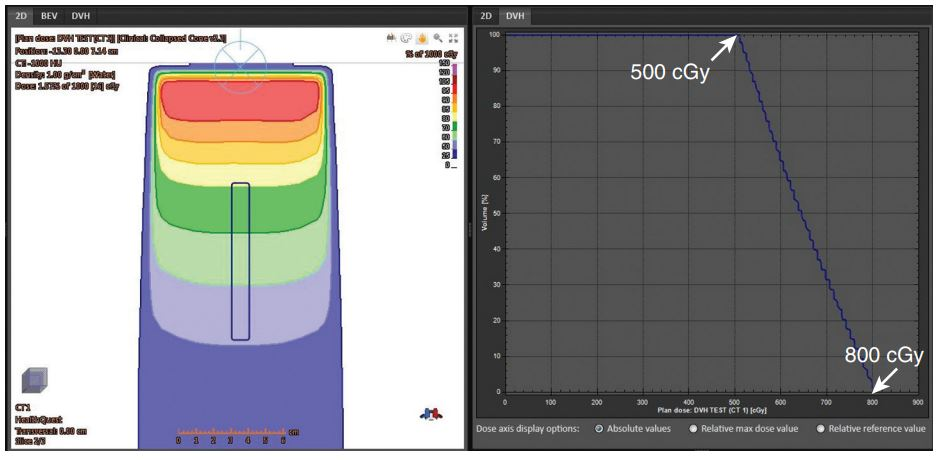
\includegraphics[width=0.8\textwidth]{Imagens/exemploQaDvh.JPG}
		}%
		\caption{Exemplo de QA do DVH}
		\label{fig:exemploQaDvh}
	\end{figure}

	Para sistemas de \textcolor{MediumOrchid}{\textbf{\textit{braquiterapia}}}, esta validação pode ser simples. Ao colocar uma fonte pontual no centro de uma estrutura esférica, uma relação dose-volume muito previsível pode ser determinada. 
	
	A importância do \textcolor{MediumOrchid}{\textbf{\textit{tamanho da grade de cálculo dose}}} deve ser avaliada. Isso pode ser feito \textcolor{MediumOrchid}{\textbf{\textit{observando as mudanças de volume de dose por tamanho de grade para estruturas de vários volumes}}}. Isso vale para qualquer tipo de sistema, não apenas para a braquiterapia. Se pequenos volumes devem ser avaliados, tamanhos de grade menores podem ser necessários. Isso dependerá dos algoritmos de interpolação do sistema e do método pelo qual os voxels são atribuídos às estruturas.

	O exemplo da \ref{fig:efeitoDaGradeDeCalculoNoDVH} mostra as diferenças de efeito com base no tamanho e localização da estrutura. A estrutura menor perto da borda do feixe (alto gradiente) tem a mudança mais dramática quando a grade de dose é alterada de 4 mm para 1 mm. Exemplos clínicos disso podem ser o quiasma óptico ou o bulbo peniano.

	\begin{figure}[h]
		\centering
		\fcolorbox{DarkTurquoise}{white}{%
			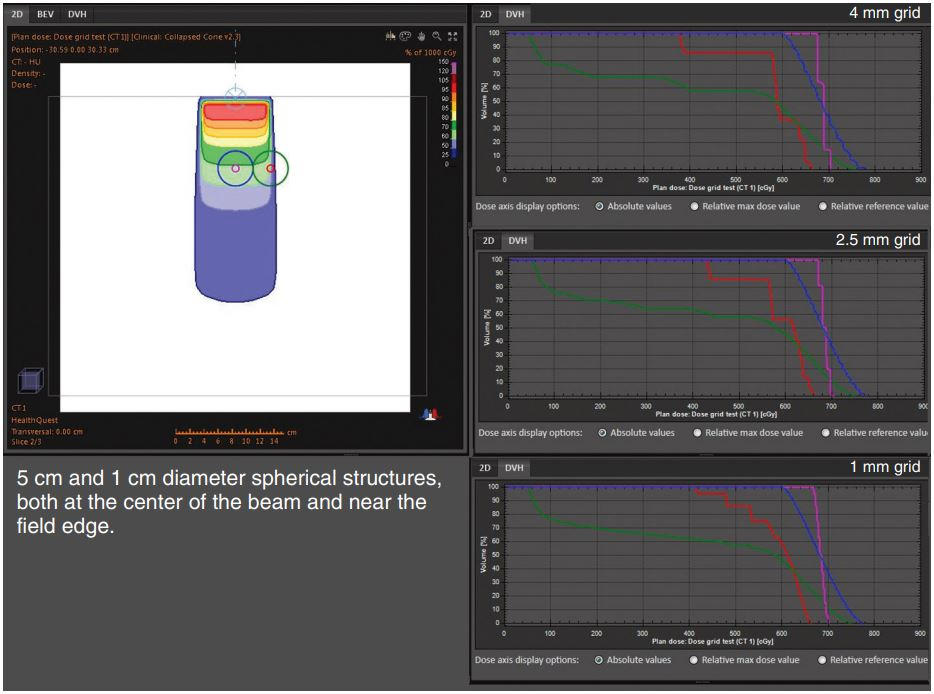
\includegraphics[width=0.8\textwidth]{Imagens/efeitoDaGradeDeCalculoNoDVH.JPG}
		}%
		\caption{O efeito do tamanho da grade no cálculo de DVH.}
		\label{fig:efeitoDaGradeDeCalculoNoDVH}
	\end{figure}

\subsection*{Testes Não-Dosimétricos}

	O AAPM TG-53 e IAEA TRS-430 descrevem em detalhes os testes não dosimétricos recomendados. Além disso, o AAPM TG-201, \textit{``Quality Assurance of External Beam Treatment Data Transfer''}, descreve o teste de transferência de dados. Uma lista de parâmetros a serem verificados incluiria: \textcolor{MediumOrchid}{\textbf{\textit{representação anatômica do paciente, contorno, autocontorno, determinação de volume, determinação de densidade, exibição de imagem, exibição de dose, sistemas de coordenadas, descrição da máquina, capacidades da máquina, parâmetros da máquina, convenções de leitura (ou seja, Comissão Eletrotécnica Internacional (IEC)), exibição de abertura, modelagem automática de campo, exibição de geometria de feixe, SSD e importação/exportação de dados}}}.

	\begin{itemize}[label=\textcolor{CarnationPink}{$\star$}]
		\item O \textcolor{DarkTurquoise}{\textbf{\textit{teste de autocontorno}}} pode ser feito usando materiais de diferentes densidades de tamanho e forma conhecidos. Por exemplo, uma esfera de acrílico dentro de um recipiente com água pode ser tomografada e depois contornada no TPS. O mesmo teste pode ser usado para determinar a precisão da densidade física/eletrônica e do volume da região em questão relatados pelo TPS. Um teste mais elaborado envolveria o uso de plásticos de diferentes densidades que se aproximam da densidade da água para testar a diferença mínima de contraste que o algoritmo pode detectar.
		
		\item O \textcolor{DarkTurquoise}{\textbf{\textit{teste de display da imagem}}} pode ser feito testando objetos de tamanho e forma conhecidos. Uma bola de boliche é um exemplo de objeto de teste que pode ser usado para testar a precisão do BEV, DRR e SSD. Por design, as bolas de boliche precisam ser perfeitamente esféricas e são ideais para esses propósitos. Obtenha uma tomografia computadorizada da bola e importe-a para o TPS. Coloque muitos feixes no centro da bola com um tamanho de campo igual ao diâmetro da bola usando diferentes combinações de ângulos de gantry, colimador e mesa. Como a bola é esférica, BEV, DRR e SSD devem ser idênticos para cada feixe. Deve-se utilizar um número idêntico de MU em cada campo e pode ser usado como parte do teste dosimétrico. Placas de phantoms podem ser utilizadas de forma semelhante. Phantoms mais elaborados também estão disponíveis, como os phantoms Quasar da Modus Medical, os phantoms Baltas da Pi Medical Research e o phantom ISIS da Radiation Products Design.
		
		\item A \textcolor{DarkTurquoise}{\textbf{\textit{precisão dos sistemas de coordenadas e orientação do paciente}}} podem ser verificados colocando marcadores nas placas utilizadas como phantom em locais conhecidos (ou seja, anterior esquerdo) e, em seguida, digitalizando e importando para o TPS para confirmar que a localização dos marcadores está correta (que está na posição anterior esquerda). O phantom DOVe da Integrated Medical Technologies é gravado com texto e objetos que tornam a determinação da orientação da imagem óbvia para qualquer orientação. Além disso, existem furos em coordenadas conhecidas para confirmar a precisão do sistema de coordenadas. Um exemplo com a imagem do phantom é apresentada na \ref{fig:phantomOrientacaoPaciente}.
		
		\begin{figure}[!h]
			\centering
			\fcolorbox{DarkTurquoise}{white}{%
				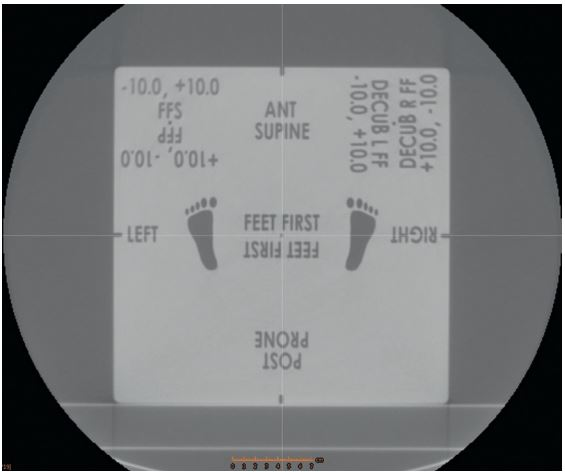
\includegraphics[width=0.6\textwidth]{Imagens/phantomOrientacaoPaciente.JPG}
			}%
			\caption{Phantom para verificação da orientação do paciente}
			\label{fig:phantomOrientacaoPaciente}
		\end{figure}
	
		\item O \textcolor{DarkTurquoise}{\textbf{\textit{teste de conectividade}}} é importante para garantir a precisão das informações em todas as etapas do processo. Os dados de imagem podem vir de dentro do departamento, de um sistema de arquivamento e comunicação de imagens (PACS - Picture Archiving and Communication system) ou de mídia provenientes de instalações externas. Os dados podem ser transferidos diretamente para o TPS ou primeiramente para um sistema de contorno. Do TPS, os dados podem ser enviados para o sistema Record \& Verify (R\&V) e um segundo sistema de verificação. Uma matriz de transferência de dados pode ser criada conforme mostrado na \ref{fig:matrixTransferenciaDados}. A matriz lista as fontes e os destinos das informações, e uma descrição dos tipos de dados é mostrada em cada célula da matriz. As células são preenchidas apenas para transferências usadas, portanto, muitas podem estar em branco. Isso ajudará a orientar o que deve ser testado. Por exemplo, em uma transferência de TC para TPS, a precisão geométrica, as informações de densidade e a orientação devem ser verificadas. Para uma transferência de TPS para R\&V, os parâmetros do feixe, as informações da sequência da lâmina e as informações da dose devem ser verificadas. Para todas as transferências, as informações de identificação do paciente devem ser verificadas.
		
		\begin{figure}[!h]
			\centering
			\fcolorbox{DarkTurquoise}{white}{%
				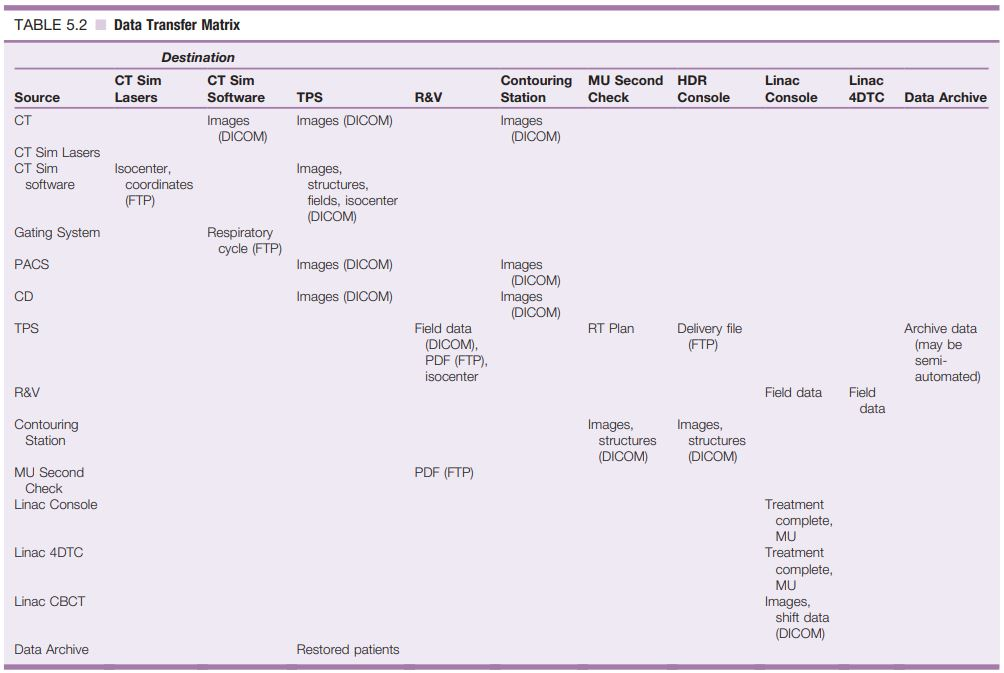
\includegraphics[width=0.8\textwidth]{Imagens/matrixTransferenciaDados.JPG}
			}%
			\caption{Matriz de Transferência de Dados}
			\label{fig:matrixTransferenciaDados}
		\end{figure}
	
		\item \textcolor{DarkTurquoise}{\textbf{\textit{Diferentes capacidades da máquina devem ser verificadas}}}, como over-travel máximo da lâmina do MLC, velocidades máximas e mínimas do gantry ou MU mínima para filtros dinâmicas. É importante verificar essas configurações para que não sejam criados planos que não possam ser entregues. Uma área que muitos sistemas TPS podem melhorar é a detecção de colisão. Agora, mais sistemas permitem a inserção da mesa de tratamento no conjunto de dados da imagem, o que ajuda a determinar onde podem ocorrer colisões. Uma estrutura cilíndrica pode ser criada com um diâmetro igual ao tamanho efetivo do “bore” do linac para visualizar a zona segura. Isso pode ser registrado criando uma tabela de ângulos de feixe permitidos com base na altura e rotação da mesa.
	
	\end{itemize}

\subsection*{Testes Específicos para Braquiterapia}

	Para o cálculo da dose de braquiterapia, a maioria dos sistemas usa o formalismo AAPM TG-43. Os sistemas calculam com base na densidade única da água e não levam em conta a falta de homogeneidade do tecido. A \textcolor{MediumOrchid}{\textbf{\textit{validação dos parâmetros de input}}} pode ser feita utilizando as referências listadas no site do IROC conforme mostra a \ref{fig:benchmarkdata}. 
	
	As referências também mostram valores de dose em vários pontos em torno de uma força de fonte de 1 U, que pode ser usada para validar o cálculo da dose. AAPM TG-138, \textit{``A Dosimetric Uncertainty Analysis for Photon-Emitting Brachytherapy Sources''}, discute as incertezas na medida da força da fonte e os parâmetros do AAPM TG-43. Eles recomendam como um consenso o uso dos valores para os parâmetros do AAPM TG-43 porque o uso de outros valores ou de vários investigadores aumentará a incerteza das doses calculadas.

	Como a orientação da semente pode não ser conhecida com precisão em um \textcolor{MediumOrchid}{\textbf{\textit{implante de semente da próstata}}}, os cálculos para sementes geralmente são feitos usando um modelo de fonte pontual, exceto se especificado de outra forma em um protocolo de ensaio clínico. Portanto, o fator de anisotropia (valor médio) é usado em vez de uma função de anisotropia que descreve a mudança na taxa de dose versus o ângulo em relação ao eixo da semente. Para \textcolor{MediumOrchid}{\textbf{\textit{braquiterapia HDR}}}, a orientação é conhecida porque o caminho do cateter é inserido no sistema para cálculo preciso da dose.
	
	Em ambos os casos, a implementação adequada deve ser verificada, \textcolor{MediumOrchid}{\textbf{\textit{checando a taxa de dose em várias distâncias e ângulos em relação ao eixo da semente}}}. Uma vez que a distribuição de dose é verificada para uma única fonte, a precisão para múltiplas fontes deve ser avaliada. Algumas áreas de desenvolvimento recente no cálculo da dose em braquiterapia são o uso de algoritmos de Monte Carlo (tanto para o cálculo dos parâmetros AAPM TG-43 quanto para o cálculo direto), incorporação de correções de heterogeneidades e contabilização do tempo de trânsito. O AAPM TG-186, \textit{``Model-Based Calculations in Brachytherapy''}, recomendou a transição do formalismo AAPM TG-43 para algoritmos de cálculo de dose baseados em modelo (MBDCA).

\section{QA ao longo da utilização do TPS}

	Após o comissionamento do TPS, a rotina de controle de qualidade deve ser estabelecida para garantir a precisão contínua do sistema. Tanto a funcionalidade do sistema quanto a integridade do modelo do feixe devem ser verificados. Normalmente, a integridade do modelo do feixe é verificada usando uma função de soma de verificação nos arquivos de dados. O AAPM TG-53 recomenda que, pelo menos uma vez a cada 12 meses ou após uma atualização de software, um subconjunto de testes dosimétricos e não dosimétricos seja realizado. Um exemplo de testes é mostrado na \ref{fig:qaTps}. Ao executar o controle de qualidade após uma atualização, é melhor revisar as notas de versão e projetar testes específicos para quaisquer alterações na funcionalidade.

	\begin{figure}[h]
		\centering
		\fcolorbox{DarkTurquoise}{white}{%
			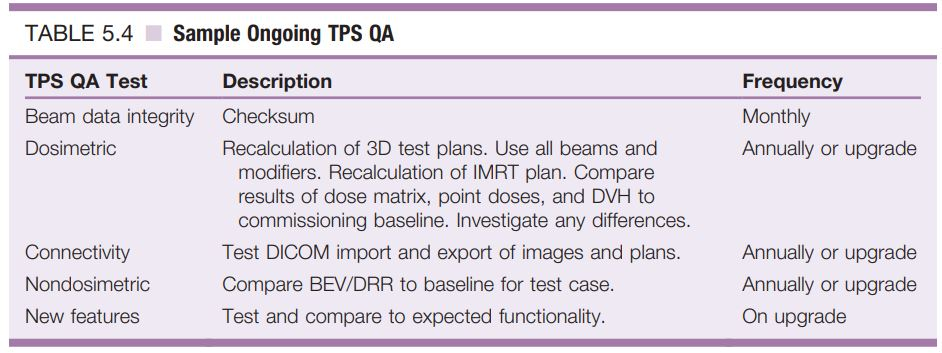
\includegraphics[width=0.8\textwidth]{Imagens/qaTps.JPG}
		}%
		\caption{Exemplo de controle de qualidade contínuo do TPS}
		\label{fig:qaTps}
	\end{figure}

\section{QA Paciente-Específico}

	O controle de qualidade Paciente-Específico se enquadra em duas categorias:

	\begin{enumerate}[label=\textcolor{CarnationPink}{\roman*.}]
		\item Para verificação do cálculo de MU do TPS;
		\item Para validação de distribuições de dose de IMRT.
	\end{enumerate}

	Primeiro, o cálculo de MU do TPS deve ser verificado por um método independente, conforme recomendado pelas Diretrizes Práticas ACR-ASTRO. Isso normalmente é feito comparando com o cálculo de outro sistema e é descrito na seção 5.3.4 do AAPM TG-114. A \ref{fig:niveisAcaoMu} mostra os níveis de ação sugeridos pelo AAPM TG-114 para discordância entre a verificação e os cálculos primários, incluindo heterogeneidade.
	
	\begin{figure}[h]
		\centering
		\fcolorbox{DarkTurquoise}{white}{%
			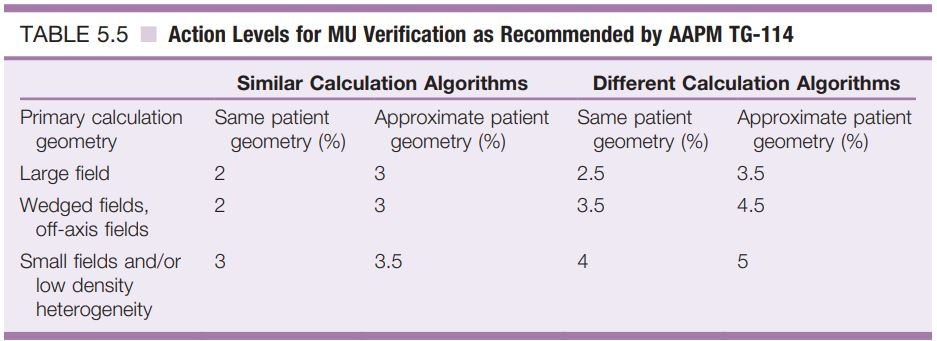
\includegraphics[width=0.8\textwidth]{Imagens/niveisAcaoMu.JPG}
		}%
		\caption{Níveis de Ação}
		\label{fig:niveisAcaoMu}
	\end{figure}

	O AAPM TG-71,\textit{``Monitor Unit Calculations for External Photon and Electron Beams,''}, e o booklet 6 da ESTRO, \textit{``Monitor Unit Calculation for High Energy Photon Beams: Practical Examples''}, também são boas referências sobre verificação de MU. Se a verificação da UM for feita por \textcolor{MediumOrchid}{\textbf{\textit{cálculo manual}}}, o AAPM TG-71 fornece uma descrição detalhada da metodologia. \textcolor{MediumOrchid}{\textbf{\textit{Os fatores incluídos no cálculo são taxa de dose de referência, espalhamento do colimador, espalhamento phantom, profundidade, modificadores de feixe, razões off-axis e distância}}}. Selecionar um ponto de cálculo apropriado é importante. Devem ser evitados, por exemplo, pontos blindados a cerca de 2 cm da borda do campo ou a 1 cm de uma interface heterogênea. Pode não ser possível usar o mesmo ponto para todos os campos de um plano.

	A segunda categoria é a \textcolor{MediumOrchid}{\textbf{\textit{validação das distribuições de dose IMRT}}}. Originalmente, isso envolvia o uso de uma \textcolor{MediumOrchid}{\textbf{\textit{câmara de ionização}}} para verificar a \textcolor{MediumOrchid}{\textbf{\textit{dose absoluta}}} e o \textcolor{MediumOrchid}{\textbf{\textit{filme}}} para verificar a \textcolor{MediumOrchid}{\textbf{\textit{precisão espacial}}}. Posteriormente, as \textcolor{MediumOrchid}{\textbf{\textit{matrizes de detectores}}} se tornaram a ferramenta mais amplamente adotada para essa verificação. Em qualquer um dos métodos, \textcolor{MediumOrchid}{\textbf{\textit{a fluência do paciente é recalculada em um phantom}}} no qual os dispositivos de medida são colocados. As doses recalculadas no phantom são então comparadas com as medidas realizadas no phantom.

	O método de avaliação mais comum é o \textcolor{MediumOrchid}{\textbf{\textit{índice gama}}} originalmente descrito por Low e Dempsey. Esse método usa os critérios de diferença de dose e distância em conjunto para avaliar a diferença entre as doses planejadas e medidas ponto a ponto. Isso permite que diferentes critérios sejam usados em diferentes áreas da distribuição de dose com base no gradiente nessa área. \textcolor{MediumOrchid}{\textbf{\textit{A diferença de dose é usada para as áreas de baixo gradiente, e a distância de concordância é usada em áreas de alto gradiente}}}. Os resultados geralmente são relatados como a porcentagem de pontos que passam em uma combinação dos dois critérios (ou seja, 95\% dos pontos que passam no critério de 2\%/2 mm). 
	
	Existe alguma controvérsia sobre como os feixes devem ser medidos (gantry fixo versus ângulos clínicos, campo a campo versus campos compostos) e quais critérios usar. Se ângulos ou arcos clínicos do gantry estiverem sendo medidos, a dependência angular do dispositivo de medição deve ser cuidadosamente caracterizada. Se utilizar o método de índice gama padrão, muitas instituições usam um critério de 3\%/3 mm ou mesmo 5\%/5 mm; no entanto, foi demonstrado que isso pode não detectar erros significativos. Na ausência de um padrão, cada instituição deve determinar seus próprios critérios com base nas deficiências conhecidas no sistema da instituição. AAPM TG-119 sugere que esses limites devem ser estabelecidos com base na determinação da variabilidade estatística na prática clínica. O \textcolor{MediumOrchid}{\textbf{\textit{critério de 3\%/3 mm}}} seria um limite superior razoável, com 2\%/2 mm como alternativa. O AAPM TG-120 sobre ferramentas e técnicas de dosimetria para IMRT fornece uma descrição dos dosímetros, phantoms e técnicas de análise em uso. 
	
	Outros dispositivos também estão começando a ser usados, incluindo dosimetria de portal imager e arrays de detectores 3D. A \ref{fig:detectoresQaPacienteEspecifico} mostra algumas matrizes de detectores comumente usadas para controle de qualidade específico do paciente. Além disso, outras metodologias que omitem qualquer medida foram propostas e utilizadas em alguns centros. Isso envolve o recálculo da dose com base no sequenciamento de lâminas do MLC. Embora isso confirme o cálculo da dose, ele remove o controle de qualidade do hardware. Nesse caso, a instituição deve ter um rigoroso programa de controle de qualidade do MLC.

	\begin{figure}[h]
		\centering
		\fcolorbox{DarkTurquoise}{white}{%
			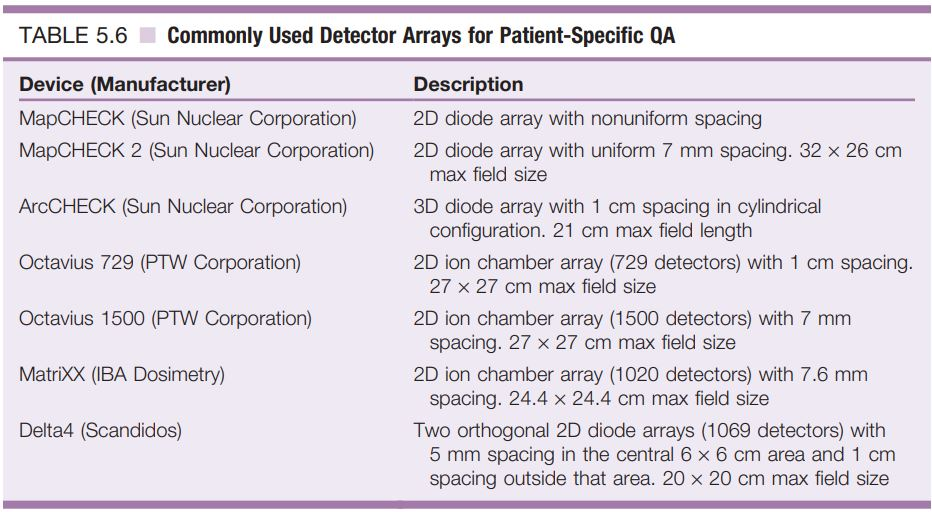
\includegraphics[width=0.8\textwidth]{Imagens/detectoresQaPacienteEspecifico.JPG}
		}%
		\caption{Matrizes de detectores comumente usadas para controle de qualidade específico do paciente}
		\label{fig:detectoresQaPacienteEspecifico}
	\end{figure}


\section{Resumo}

	O cálculo preciso da dose durante o planejamento do tratamento é fundamental para atingir os objetivos do tratamento. A primeira etapa envolve a caracterização da fonte de radiação no sistema de planejamento de tratamento (linac ou braquiterapia), verificando os parâmetros consensuais que descrevem a fonte ou medindo os parâmetros apropriados da fonte para a modelar com precisão. Feito isso, outras medidas e/ou cálculos devem ser feitos para validar o modelo de cálculo. 

	As comparações podem ser feitas usando outra metodologia de cálculo independente, como Monte Carlo, ou usando dados de referência publicados para a mesma fonte. Uma etapa importante no processo de validação é um teste abrangente de todo o processo clínico chamado de teste de ponta a ponta (end-to-end). Isso envolve o uso de phantoms de pacientes com dosímetros embutidos que são submetidos ao mesmo processo que um paciente real, com cada tarefa sendo executada pelo membro da equipe que a executaria em um paciente. Desta forma, todo o processo pode ser avaliado quanto à precisão da dose e precisão geométrica. Algumas questões que devem ser abordadas no teste dosimétrico são:

	\begin{enumerate}[label=\textcolor{CarnationPink}{\roman*.}]
		\item Cálculo em condições padrão (campos quadrados ou retangulares em diferentes SSDs para um phantom homogêneo);
		\item Cálculo em cenários clínicos (feixes oblíquos, materiais não homogêneos, irregularidade de superfície, flash da pele, falta de equilíbrio de espalhamento, modulação de feixe);
		\item Cálculos de volume de dose. Muitos julgamentos clínicos são baseados nas informações do volume da dose e é fundamental que sejam precisos.
		\item Controle de qualidade específico do paciente. Isso envolve a verificação do feixe MU ou tempo de tratamento e a validação da dose absoluta e precisão geométrica dos feixes modulados (IMRT).
	\end{enumerate}

	Além da precisão dosimétrica de um TPS, os componentes não dosimétricos do sistema devem ser avaliados quanto à precisão. Esses incluem:

	\begin{enumerate}[label=\textcolor{CarnationPink}{\roman*.}]
		\item Representação anatomica do paciente;
		\item Contorno manual e automático;
		\item Determinação volumétrica;
		\item Determinação da densidade;
		\item Exibição da imagem;
		\item Exibição da dose;
		\item Exibição da abertura de campo;
		\item Exibição da geometria do feixe;
		\item Sistemas de Coordenadas;
		\item Descrições da Máquina (limites e parâmetros)
		\item Convenções de Leituras (IEC)
		\item SSD
		\item Import e Export dos dados
	\end{enumerate}

	Todos esses testes levam um tempo considerável e isso deve ser levado em consideração na implementação de um novo sistema. Normalmente, isso pode levar de 6 a 8 semanas de dias de trabalho padrão de 8 horas. Em clínicas menores com recursos limitados, pode ser necessário empregar estratégias alternativas para uma implementação tranquila sem interromper o fluxo de trabalho clínico. Isso pode envolver o uso de pessoal de física contratado temporariamente ou uma liberação escalonada de recursos de equipamentos, um feixe de energia por vez, por exemplo.

	Uma vez que o sistema tenha sido comissionado, a precisão contínua deve ser assegurada pela implementação de um processo contínuo de controle de qualidade. Isso envolverá o cálculo da dose e exibição de informações para casos de referência para os quais as linhas de base foram estabelecidas durante o comissionamento. Um subconjunto de testes também deve ser executado após atualizações do software.

	O ICRU recomenda que o cálculo da dose absorvida seja preciso com 5\% de incerteza. À medida que mais dados são acumulados em relação à resposta à dose, é imperativo que as doses calculadas sejam tão precisas quanto possível para que relações significativas possam ser determinadas. O comissionamento preciso e o controle de qualidade do TPS são essenciais para atingir esse objetivo.


\bibliography{ref.bib}
\end{document}